%\documentclass[handout]{rsuqbeamernew}
\documentclass{rsuqbeamernew}
\def\ANIMATE{0}   %   0/1: Compile animations or not

%%%%%%%%%%%%%%%%%%%%%%%%%%%%%%%%%%%%%%%%%%%%%%%%%%%%%%%%%%%%%%%%%%%%%%%%%%%%%%%%%%%%%%%%%%%%%%%%%%%%%%
%
%
%
\title[HPC Meeting]{Dispatcher Restart}
\subtitle{HPC Meeting}
\institute[Chair of Risk \& Safety] {}
\author[D. Wicaksono]{Damar Wicaksono}

\date[December 03, 2019] {\small December 03, 2019}

% graphics
\graphicspath{{Figures/},{Figures/Christos/}}

\usepackage{bstnotations}
\usepackage[noend]{algpseudocode}
\usepackage{algorithm}
\usepackage{animate}


% additional
\newcommand{\card}[1]{\mathrm{card}(#1)}
\DeclareMathOperator*{\argmax}{arg\,max}
\DeclareMathOperator*{\argmin}{arg\,min}

% algorithm abbreviations
\newcommand{\Ntot}{\textsc{Ntot}}
\newcommand{\Ninit}{\textsc{Ninit}}
\newcommand{\M}{\textsc{M}}
\newcommand{\Nneigh}{\textit{NNeighbour}}
\newcommand{\NBound}{\textsc{NBoundaries}}
\newcommand{\NneighThresh}{\textsc{NNeighbourThreshold}}
\newcommand{\Penal}{\textit{Penalization}}
\newcommand{\Pmax}{\textsc{Pmax}}
\newcommand{\NRefine}{\textsc{NRefine}}
\newcommand{\NRefineIter}{\textsc{NEnrIter}}
\newcommand{\Func}[1]{\textsc{model}(#1)}
\newcommand{\Inp}[1]{\textsc{input}(#1)}
\newcommand{\X}{\textit{X}}
\newcommand{\Xcurr}{\textit{Xcurr}}
\newcommand{\Xnew}{\textit{Xnew}}
\newcommand{\Y}{\textit{Y}}
\newcommand{\Ycurr}{\textit{Ycurr}}
\newcommand{\Ynew}{\textit{Ynew}}
\newcommand{\PCEref}{\textit{PCEpar}}
\newcommand{\Dref}{\textit{Dpar}}
\newcommand{\Di}{\textit{Di}}
\newcommand{\Dcand}{\textit{Dcand}}
\newcommand{\Dfirst}{\textit{D1}}
\newcommand{\Dsec}{\textit{D2}}
\newcommand{\Dnew}{\textit{Dchild}}
\newcommand{\Res}{\textit{Resid}}
\newcommand{\Rescurr}{\textit{ResidualCurr}}
\newcommand{\Errors}[1]{\textit{Errors}#1}
\newcommand{\ErrorLoo}{\textit{ErrorLOO}}
\newcommand{\Domain}[1]{\textit{Domains}#1}
\newcommand{\PCEs}[1]{\textit{PCEs}#1}
\newcommand{\PCEnew}{\textit{PCEchild}}
\newcommand{\RefineDom}[1]{{\altx \textsc{getRefineDomain}}(#1)}
\newcommand{\ConstrPCE}[1]{{\altx \textsc{constructPCE}}(#1)}
\newcommand{\EnrExpD}[1]{\textsc{enrichDesign}(#1)}
\newcommand{\ConstrSSE}[1]{\textsc{constructSSE}(#1)}
\newcommand{\Size}[1]{\textsc{getSize}(#1)}
\newcommand{\Volume}[1]{\textsc{getVolume}(#1)}
\newcommand{\EvalSSE}[1]{\textsc{evaluateSSE}(#1)}
\newcommand{\ComputeError}[1]{\textsc{estimateError}(#1)}
\newcommand{\SplitDomain}[1]{{\altx \textsc{splitDomain}}(#1)}
\newcommand{\SelectRefine}[1]{{\altx \textsc{selectRefine}}(#1)}
\newcommand{\degC}{\ensuremath{\,^{\circ}\mathrm{C}}}
\newcommand{\BParams}{1}
\newcommand{\Bparams}{1}
\newcommand{\Bprior}{1}
\newcommand{\Bcond}{1}
\newcommand{\Bevi}{1}

% algorithm environment
\algnewcommand{\Inputs}[1]{%
	\State \textbf{inputs:}
	\vspace{-1em}
	\Statex \hspace*{\algorithmicindent}\parbox[t]{0.96\linewidth}{\raggedright 
		#1}
}
\algnewcommand{\Repeater}[1]{%
	\State \textbf{repeat:}
	\vspace{-1em}
	\Statex \hspace*{\algorithmicindent}\parbox[t]{0.96\linewidth}{\raggedright 
		#1}
}

\algnewcommand{\Initialize}[1]{%
	\State \textbf{initialize:}
	\vspace{-1em}
	\Statex \hspace*{\algorithmicindent}\parbox[t]{0.96\linewidth}{\raggedright 
		#1}
}


%%%%%%%%%%%%%%%%%%%%%%%%%%%%%%%%%%%%%%%%%%%%%%%%%%%%%%%%%%%%%%%%%%%%%%%%%%%%%%%%%%%%%%%%%%%%%%%%%%%%%%
\begin{document}

%----------------------------------------------------------------------------------------------------
\begin{frame}[t]{Motivation - surrogate modeling}
	\small
	\Tit{Typical problem}\\
	\begin{itemize}
		\item [] Consider a {\altx computational model} $\cm$ with input 
	\end{itemize}
	\emphconc{Uncertainty propagation}
	\begin{minipage}[t][3cm][t]{\textwidth}
	%	\includegraphics[width=\textwidth]{InverseProblem_1}
	\end{minipage}	

	\pause
	\Tit{Difficulties}
	\begin{itemize}
		\item {\altx Complex local 
		characteristics} and {\altx non-smoothness} difficult for {\altx 
		global} surrogate models
		\item Propose assembly of {\altx local} surrogate models
		\item Employ {\altx polynomial chaos expansion} (PCE) 
	\end{itemize}
	
\end{frame}

%----------------------------------------------------------------------------------------------------

%----------------------------------------------------------------------------------------------------
\section{Surrogate modeling}
\secoutline


%----------------------------------------------------------------------------------------------------
\subsection{Polynomial chaos expansion}
\begin{frame}[t]{Polynomial chaos expansion (PCE)}
	\small
	\begin{itemize}
		\item[] If $\BParams\sim\prod_{i=1}^M\pi(x_i)$ ({\altx independent}), 
		express square integrable $\cm$ in a {\altx sparse} orthogonal 
		{\altx polynomial 
		basis} 
		$\{\Psi_{\ve{\alpha}}\}_{\ve{\alpha}\in\mathbb{N}^M}$:
	\end{itemize}
	
	\begin{block}{PCE representation \hfill
			\refcite{white}{Xiu \& Karniadakis, SIAM journal on scientific 
			computing (2002)}}
		\begin{equation*}
		\cm(\BParams) =
		\sum_{\ve{\alpha}\in\ca}a_{\ve{\alpha}}\Psi_{\ve{\alpha}}(\BParams) + 
		\mathcal{R}(\BParams)
		\end{equation*}
		
		\begin{itemize}
			\itemsep0.5em
			\item[] truncated set $\ca\subset\mathbb{N}^M$, coefficients 
			$a_{\ve{\alpha}}$ 
		\end{itemize}
	\end{block}
	
	\Tit{Practical computation} (regression approach)
	\begin{itemize}
		\itemsep0.5em
		\item {\altx Experimental design} $\cx$ and $\cm(\cx)$
		\item Least angle regression ({\altx LARS})
		\item Basis {\altx adaptivity} with $\varepsilon_{\mathrm{LOO}}$\hfill
		\refcite{Green4}{Blatman \& Sudret, Journal of Computational Physics 
		(2011)} 
	\end{itemize}
	\pause
	\vspace{1em}
	\emphconc{Can we extract more information from residual?}
\end{frame}

%----------------------------------------------------------------------------------------------------
\subsection{Stochastic spectral embedding}
\begin{frame}[t]{Stochastic spectral embedding (SSE)}
	\small
	\Tit{Idea}\\
	Approximate $\mathcal{R}()$ with two PCEs in {\altx equal-sized
	subdomains}\\
	\pause
	\begin{minipage}{0.65\linewidth}
		\Tit{Proposed approach}\\
		\begin{enumerate}
			\item $\cm(\BParams) \approx f_0^{\mathrm{PC}}(\BParams)$
			\item $\cm(\BParams) \approx 
			f_0^{\mathrm{PC}}(\BParams) + f_1^{\mathrm{PC}}(\BParams) + 
			f_2^{\mathrm{PC}}(\BParams)$
			\item $\cm(\BParams) \approx 
			f_0^{\mathrm{PC}}(\BParams) + f_1^{\mathrm{PC}}(\BParams) + 
			f_2^{\mathrm{PC}}(\BParams) + \dots$
		\end{enumerate}
	\end{minipage}
	\hfill
	\begin{minipage}{0.34\linewidth}
		%\includegraphics[width=\textwidth]{SSESample}
	\end{minipage}
	\pause
	\begin{block}{SSE representation}
		\begin{equation*}
		\cm(\BParams) \approx \sum_{k\in\ck}f_k^{\mathrm{PC}}(\BParams), \quad 
		\text{with} \quad f^{\mathrm{PC}}_k(\BParams) \eqdef 
\sum_{\ve{\alpha}\in\ca^k}a_{\ve{\alpha}}^k\ve{\Psi}_{\ve{\alpha}}^k(\BParams)
		\ve{1}_{\cd_{\BParams}^k}(\BParams)
		\end{equation*}
		
		\begin{itemize}
			\itemsep0.5em
			\item[] {\altx polynomial 
				basis} $\{\Psi^k_{\ve{\alpha}}\}_{\ve{\alpha}\in\mathbb{N}^M}$ 
				
		\end{itemize}
	\end{block}
\end{frame}

\begin{frame}[t]{SSE - refinement domain}
	\small
	\begin{minipage}{0.65\linewidth}
		\Tit{Problem}
		\begin{itemize}
			\item[] At every {\altx refinement} step, $\card{\ct}$ available 
			refinement domains from $\ct\subseteq\ck$
		\end{itemize}
		\vspace{1em}
		\emphconc{Which domain to focus on next?} 
		\Tit{Leave-one-out error}\\
	\end{minipage}
	\hfill
	\begin{minipage}{0.34\linewidth}
		%\includegraphics[width=\textwidth]{SSESample_terminal}
	\end{minipage}
	\pause
	\vspace*{-1em}
	\begin{itemize}
		\item[] Estimate generalization error of SSE 
		$\varepsilon_{\mathrm{GEN}}\eqdef\Esp{(\cm-\cm^{\mathrm{SSE}})^2}$ by:
	\end{itemize}
	 \begin{equation*}
	   \varepsilon_{\mathrm{LOO}} \eqdef 
	   \sum_{k\in\mathcal{T}}c_k\varepsilon_{\mathrm{LOO}}^k, 
	 \end{equation*}
	 \begin{itemize}
	 \item $\varepsilon_{\mathrm{LOO}}^k$: {\altx absolute leave-one-out 
	     error} of the $k$-th PCE
	 \end{itemize}
 	\pause
 	\emphconc{Select $k_{\mathrm{ref}} = 
 	\argmax_{k\in\ct}{c_k\varepsilon_{\mathrm{LOO}}^k}$} 
\end{frame}

\begin{frame}[t]{SSE - splitting direction}
	\small
	\begin{columns}
		\begin{column}{0.7\textwidth}
		\Tit{Problem}
		\begin{itemize}
			\item[] In selected domain $k_{\mathrm{ref}}$
		\end{itemize}
		\emphconc{Which of the {\altx M} dimensions to split along?} 
		\pause
		\Tit{Partial variance}\\
		Measure of variability along $i$-th dimension in previous residual
		\begin{equation*}
		V_i \eqdef \Esp{\Var{f_{k_{\mathrm{ref}}}^{\mathrm{PC}}\vert X_i}}
		\end{equation*}
		\begin{itemize}
			\item Available {\altx analytically}! 
			\item Corresponds to first order {\altx Sobol' index}
		\end{itemize}
		\pause
		\emphconc{Select $i_{\mathrm{split}} = 
		\argmax_{i\in \{1,\dots,M\}}{V_i}$} 
		\end{column}
		\begin{column}{0.3\textwidth}		
			\begin{minipage}{\linewidth}
				\centering
				%\includegraphics[width=0.9\textwidth]{SSE_split_2D_domain_1}
			\end{minipage}
		\end{column}
	\end{columns}
\end{frame}

\begin{frame}[t]{Stopping criterion}
	\small
	\Tit{Track leave-one-out error}
	%\begin{center}
		%\includegraphics[width=0.7\textwidth]{Christos_convergence}
	%\end{center}
	\pause
	\Tit{Size of}
	\begin{itemize}
		\item Intuitive algorithm parameter $\NRefine$
	\end{itemize}
\end{frame}

\begin{frame}[t]{Algorithm}
	\small
	\begin{algorithmic}[0]
		\Inputs{
			\State \X, \Func{\X}, \NRefine, \Pmax, \Inp{}
		}\\
		\Initialize{
			\State
			\State $\Res\gets\Func{\X}$
			\State $\PCEs[1]\gets\ConstrPCE{\X,\Res,\Domain{[1]},\Inp{},\Pmax}$
		}\\	
		\Repeater{
		\State $\PCEref, \Dref\gets \SelectRefine{\PCEs{}, \Domain{}}$
		\State $\Dnew[1],\Dnew[2]\gets\SplitDomain{\PCEref,\Dref}$ 
		\For{$\textit{d}\gets 1, 2$}
		\If{at least $\NRefine$ samples inside $\Dnew[d]$}
		\State $\PCEnew[d]\gets\ConstrPCE{\X,\Res,\Dnew[d],\Inp{},\Pmax}$ 
		\EndIf
		\EndFor
		\State Update $\Res$, $\Domain$, $\PCEs{}$
		}
	\end{algorithmic}
\end{frame}

%----------------------------------------------------------------------------------------------------
\subsection{Application}
\begin{frame}[t]{Application - Image}
	\small
	\Tit{Image}\\
	$\Ntot=800\times 600 = 4.8\cdot 10^5$, $\NRefine=1\,000$,$\Pmax = 20$\\[1em]
	\begin{minipage}{0.49\linewidth}
		\center
		\ifthenelse{\equal{\ANIMATE}{1}}
		{ 
			\animategraphics[controls, 
			width=0.6\linewidth,]{25}{Christos_SSE_}{1}{277}
		}
		{
			\raisebox{1.5em}{
				%\includegraphics[width=0.6\linewidth]{Christos_SSE_277.png}
			}
		}\\
	\end{minipage}
	\hfill
	\begin{minipage}{0.5\linewidth}
		\center
		\raisebox{1.3em}{
	%	\includegraphics[width=0.6\linewidth]{Christos_true.png}
		}
	\end{minipage}
	\emphconc{$3.5\cdot10^4$ non-zero coefficients}
\end{frame}

\begin{frame}[t]{Application - High dimensional problem}
	\small
	\Tit{Problem}\\
	\begin{equation*}
	= \frac{10^M}{2} \left[\varphi(10\cdot(-1/3)) + 
	\varphi(10\cdot(-2/3))\right]
	\end{equation*} 
	\hfill \refcite{Green4}{Modified from Zhou, PhD Thesis (1998)}\\
	\begin{minipage}{0.49\linewidth}
		\begin{itemize}
			\item $\varphi$ proportional to {\altx multivariate normal 
			distribution}
			\item increasingly flat in higher dimensions
			\item $\sim\prod_{i=1}^M\cn(x_i\vert 0.5,0.3)$
			\item {\altx $M=50$}
		\end{itemize}
	\end{minipage}
	\hfill
	\begin{minipage}{0.49\linewidth}
	%	\includegraphics[width=\linewidth]{zhou.png}
	\end{minipage}
\end{frame}

\begin{frame}[t]{Application - High dimensional problem}
	\small
	\Tit{Results}\\
	\centering
%	\includegraphics[width=0.9\linewidth]{Zhou_RMSE}
\end{frame}

\begin{frame}[t]{SSE - flattening}
	\small
	\begin{itemize}
		\item[]  To reduce SSE {\altx size}, increase {\altx prediction speed}, 
		allow {\altx post-processing}
	\end{itemize}
	\begin{center}
	%	\includegraphics[width=0.3\linewidth]{SSESample}
		\raisebox{5em}{$\Rightarrow$}
	%	\includegraphics[width=0.3\linewidth]{SSESample_Flat}
	\end{center}
	
	\pause
	\begin{block}{SSE representation - flattened}
		\begin{equation*}
		\cm(\BParams) \approx \sum_{k\in\ck}f_k^{\mathrm{PC}}(\BParams) = 
		\sum_{k\in\ct}f_{k,T}^{\mathrm{PC}}(\BParams)
		\end{equation*}
		
		\begin{itemize}
			\item[] $f_{k,T}^{\mathrm{PC}}$ can be computed {\altx 
				analytically} from $\{f_{k}^{\mathrm{PC}}\}_{k\in\ck}$
		\end{itemize}
	\end{block}
\end{frame}

%----------------------------------------------------------------------------------------------------
\subsection{Post-processing}
\begin{frame}[t]{SSE post-processing}
	\small
	\Tit{Analytical quantities}
	\begin{itemize}
		\item [] {\altx All} PCE post-processing capabilities are preserved
	\end{itemize}
	\pause
	\begin{block}{Post-processing}
		\begin{itemize}
			\item {\altx Mean}
			\begin{equation*}
			\Esp{f^{\mathrm{SSE}}(\ve{X})} = \sum_{k\in\ck}c_ka_{\ve{0}}^{k}
			\end{equation*}
			\item {\altx Variance}\\
			After \emph{flattening} to terminal domains:			
			\begin{equation*}
			\Var{f^{\mathrm{SSE}}(\ve{X})} = 
			\sum_{k\in\ct}c_k\sum_{\ve{\alpha}\in\ca^{T}}	
			\left(a_{\ve{\alpha}}^{k,T}\right)^2 - 
			\left(\Esp{f^{\mathrm{SSE}}(\ve{X})}\right)^2
			\end{equation*}
		\end{itemize}
	Also {\altx partial variance} (Sobol' indices)
	\end{block}
\end{frame}

\begin{frame}[t]{Application - High dimensional problem}
	\small
	\Tit{Results}\\
	\begin{center}
	%	\includegraphics[width=\linewidth]{Zhou_Mean}
	\end{center}
\end{frame}

\begin{frame}[t]{Application - High dimensional problem}
	\small
	\Tit{Results}\\
	\begin{center}
	%	\includegraphics[width=\linewidth]{Zhou_Var}
	\end{center}
\end{frame}

%----------------------------------------------------------------------------------------------------
%----------------------------------------------------------------------------------------------------
\section{Bayesian model calibration}
\secoutline

\begin{frame}[t]{Motivation - Bayesian model calibration}
	\small
	\Tit{Typical problem}\\
	\begin{itemize}
		\item Calibrate {\altx computational model} $\cm$ with {\altx data} 
		$\cy$
		\item {\altx Bayesian model calibration} framework allows 
		computation of input distribution $\BParams$ conditioned on data 
		({\altx posterior})
	\end{itemize}
	%\begin{minipage}[t][3cm][t]{\textwidth}
	%	\only<1| 
	%	handout:0>{\includegraphics[width=\textwidth]{InverseProblem_1}}
	%	\only<2| 
	%	handout:0>{\includegraphics[width=\textwidth]{InverseProblem_2}}
	%	\only<3-| 
	%	handout:1>{\includegraphics[width=\textwidth]{InverseProblem_3}}
	%\end{minipage}	
	
	\visible<4>{
		\emphconc{
			In {\altx practice} the  computation of posterior quantities is 
			{\altx 
				challenging}
	}}
\end{frame}

\begin{frame}{Bayesian inversion}
	\small
	Given {\altx parameters} 
	$\BParams\sim\Bprior$ and 
	{\altx 
		measurements} 
	$\cy$, the Bayesian inverse problem reads:
	\begin{equation*}
	\pi(\Bparams\vert\cy) = \frac{\cl(\Bparams;\cy)\Bprior}{Z} 
	\quad 
	\text{where} \quad 
	Z = \int_{\cd_{\BParams}}\cl(\Bparams;\cy)\Bprior\di{\Bparams}
	\end{equation*}
	with:
	\begin{itemize}
		\item $\cl:\cd_{\BParams}\to\mathbb{R}^{+}$: {\altx 
			likelihood 
			function} (measure of how well the model fits the data) 
		\item $\pi(\Bparams\vert\cy)$: {\altx posterior} 
		density 
		function
	\end{itemize}
	
	\pause
	\begin{block}{Quantities of Interest (QoI)}
		Often one is interested in expectations of QoI {\altx following 
			calibration}:
		$h(\Bparams):\cd_{\BParams}\to\mathbb{R}$:
		\begin{equation*}
		\Esp{h(\BParams)\Bcond\cy} = 
		\int_{\cd_{\BParams}}h(\Bparams)\pi(\Bparams\Bcond\cy)\di{\Bparams}
		\end{equation*}
		\eg{}posterior moments.
	\end{block}
\end{frame}	

\begin{frame}[t]{Spectral likelihood expansions (SLE)}
	\small
	\Tit{Principle}
	\begin{equation*}
	\cl(\BParams) \approx  
	\sum_{\ve{\alpha}\in\ca}
	a_{\ve{\alpha}}\Psi_{\ve{\alpha}}(\BParams)
	\end{equation*}
	
	\pause
	\Tit{Practical implementation}
	\begin{itemize}
		\itemsep0.5em
		\item {\altx  Sparse polynomial chaos expansions} of the
		likelihood function
		\item Using {\altx basis adaptive LARS}
	\end{itemize}
	\pause 
	\begin{block}{Post-processing $a_{\ve{\alpha}}$ \hfill
			\refcite{white}{Nagel \& Sudret, J. Comput. Phys.  (2016)}}
		\begin{align*}
		Z = \Esp{\mathcal{L}(\BParams)}&\approx 
		a_{\ve{0}} \\ 
		\pi(\Bparams\Bcond\cy) &\approx 
		\Bprior\sum_{\ve{\alpha}\in\ca}
		\frac{a_{\ve{\alpha}}}{a_{\bf 0}} \Psi_{\ve{\alpha}}(\Bparams)\\
		\Esp{h(\BParams)\Bcond\cy} &\approx 
\frac{1}{a_{\ve{0}}}\sum_{\ve{\alpha}\in\ca}a_{\ve{\alpha}}b_{\ve{\alpha}}
		\quad \text{after} \quad h(\BParams)\approx 
		\sum_{\ve{\alpha}\in\ca}
		b_{\ve{\alpha}}\Psi_{\ve{\alpha}}(\BParams)
		\end{align*}
	\end{block}
\end{frame}

\subsection{SSE for Bayesian inversion}
\begin{frame}[t]{SSE for BI}
	\small
	\begin{columns}
		\begin{column}[T]{0.3\linewidth}
			\emphconc{SLE not feasible in practical Bayesian problems!}
		%	\includegraphics[width=\textwidth]{scream}
		\end{column}
		\begin{column}[T]{0.5\linewidth}
			\pause
			\Tit{Complex local characteristics}
			\begin{itemize}
				\item[] SSE more suitable
			\end{itemize}
			\vspace{1em}
			\pause
			\Tit{Compact support}
			\begin{itemize}
				\item[] Need adaptive experimental design
			\end{itemize}
			\vspace{1em}
			\pause
			\Tit{Preserve post-processing}
			\begin{itemize}
				\item[] Exploit PCE spectral nature
			\end{itemize}
			\pause
			\vspace{1em}
			\begin{block}{SSE representation of $\cl$}
				\begin{equation*}
				\cl(\BParams) \approx \sum_{k\in\ck}f_k^{\mathrm{PC}}(\BParams)
				\end{equation*}
			\end{block}
		\end{column}
	\end{columns}
\end{frame}

%------------------------------------------------------------------------------
\subsection{Post-processing}
\begin{frame}[t]{Post-processing of SSE}
	\small
	\Tit{Analytical posterior}
	\begin{itemize}
		\item[]After the construction of an SSE approximation of 
		$\mathcal{L}$, the full posterior distribution or QoI can be 
		computed analytically:
	\end{itemize}
	
	\begin{block}{Post-processing $a_{\ve{\alpha}}^k$}
		\begin{align*}
		Z = \Esp{\mathcal{L}(\BParams)}&\approx \sum_{k\in\mathcal{K}} 
		c_k a_{\ve{0}}^k, \quad 
		\text{where} 
		\quad 
		c_k = 
		\int_{\cd_{\BParams}^k}\Bprior\di{\Bparams} \\ 
		\pi(\Bparams\Bcond\cy) &\approx 
		\frac{\Bprior}{Z}\sum_{k\in\mathcal{K}}
		f_{\mathrm{PC}}^k(\Bparams)\ve{1}_{\cd_{\BParams}^k}(\Bparams)\\
		\Esp{h(\BParams)\Bcond\cy} &\approx 
		\frac{1}{\Bevi}\sum_{k\in\mathcal{K}}  c_k\cdot
		\sum_{\ve{\alpha}\in\ca^{k}}a_{\ve{\alpha}}^{k}
		b_{\ve{\alpha}}^{k}
		\quad \text{after} \quad h(\Bparams)\approx 
		\sum_{\ve{\alpha}\in\ca^k}
		b_{\ve{\alpha}}^k\Psi_{\ve{\alpha}}^k(\Bparams)
		\end{align*}
	\end{block}
\end{frame}

%----------------------------------------------------------------------------------------------------
\subsection{Ingredients of a Dispatcher?}
\begin{frame}[t]{SSH Dispatcher Unit (Current version)}
  \small
   \only<1>{
    \includegraphics[width=0.95\textwidth]{ssh_dispatcher-first_step}
  }
  \only<2>{
    \includegraphics[width=0.95\textwidth]{ssh_dispatcher-second_step}
  }
  \only<3>{
    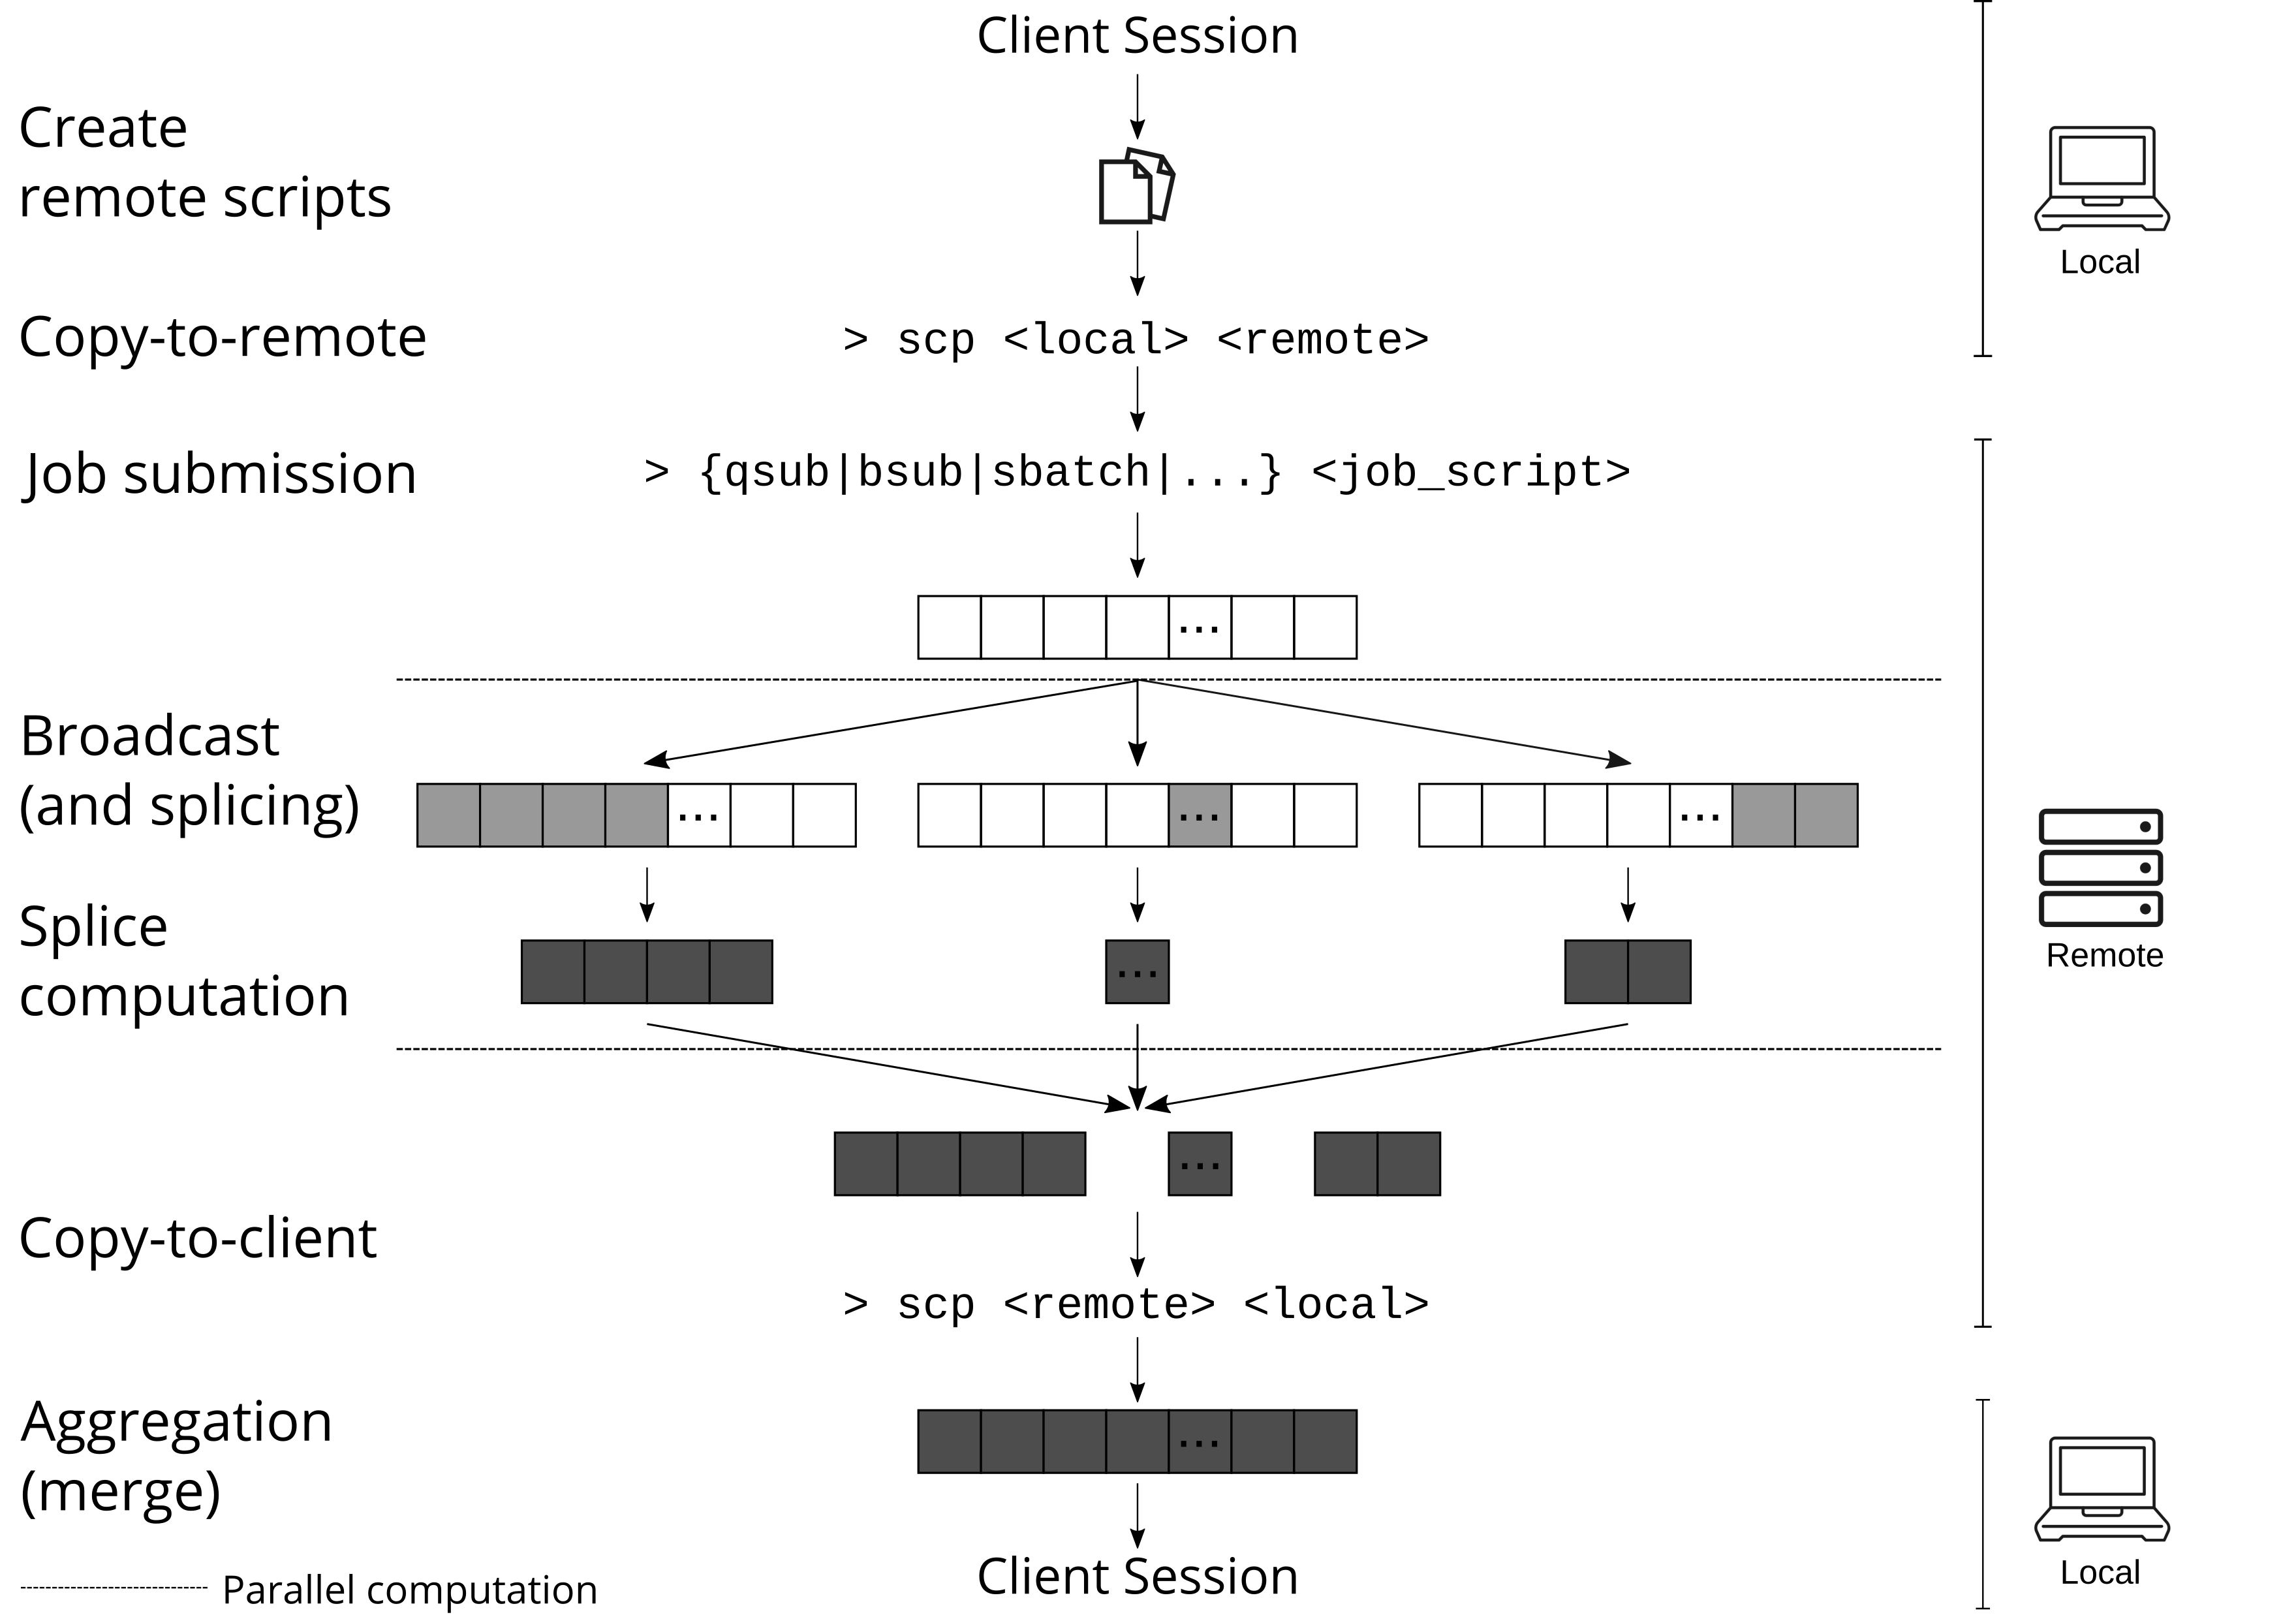
\includegraphics[width=0.95\textwidth]{ssh_dispatcher-third_step}
  }
\end{frame}


%----------------------------------------------------------------------------------------------------
\subsection{Ingredients of a Dispatcher?}
\begin{frame}[t]{Modifications to algorithm}
  \small
  \Tit{Adaptive experimental design}
  \begin{itemize}
    \item Start with $\NRefine$ points
    \item Before constructing $k$-th PCE, enrich $\cx\in\cd_{\BParams}^k$ 
    to have at least $\NRefine$ points
  \end{itemize}
  \pause
  \emphconc{Keep number of points per PCE constant}
  \vspace{2em}
  \pause
  \Tit{Splitting direction}\\
  \begin{columns}
    \begin{column}[T]{0.75\linewidth}
      \begin{itemize}
        \item Split according to {\altx residual variance}
        {\scriptsize
          \begin{equation*}
          i_{\mathrm{split}}=\argmin_{i\in\{1,\dots,M\}} \min 
          \left\{\Var{\mathcal{R}(X)}_{\cd_{\mathrm{split}}^{i,1}}, 
          \Var{\mathcal{R}(X)}_{\cd_{\mathrm{split}}^{i,2}}\right\}
          \end{equation*}
        }
      \end{itemize}
      \emphconc{Compact support}
    \end{column}
    \begin{column}[T]{0.25\linewidth}
      \only<3>{
        %\includegraphics[width=\textwidth]{SSE_split_2D_domain_1}
      }
      \only<4>{
        %\includegraphics[width=\textwidth]{SSE_split_2D_domain_2}
      }
      \only<5>{
        %\includegraphics[width=\textwidth]{SSE_split_2D_domain_3}
      }
      \only<6>{
        %\includegraphics[width=\textwidth]{SSE_split_2D_domain_4}
      }
    \end{column}
  \end{columns}
\end{frame}

\begin{frame}[t]{Adaptive Algorithm}
  \small
  \begin{algorithmic}[0]
    \Inputs{
      \State \NRefine, \Func{}, \Pmax, \Inp{}
    }\\
    \Initialize{
      \State $\Domain{[1]}\gets\cd_{\BParams}$
      \State \textcolor{red}{$\X\gets\NRefine$ samples from \Inp{}}
      \State $\Res\gets\Func{\X}$
      \State $\PCEs[1]\gets\ConstrPCE{\X,\Res,\Domain{[1]},\Inp{},\Pmax}$
    }\\	
    \Repeater{
      \State $\PCEref, \Dref\gets$ \SelectRefine{\PCEs{},\Domain{}}
      \State $\Dnew[1],\Dnew[2]\gets\SplitDomain{\PCEref,\Dref}$ 
      \For{$\textit{d}\gets 1, 2$}
      \State \textcolor{red}{$\X,\Res\gets$ enrich until at least 
        $\NRefine$ samples inside $\Dnew[d]$}
      \State $\PCEnew[d]\gets\ConstrPCE{\X,\Res,\Dnew[d],\Inp{},\Pmax}$ 
      \EndFor
      \State Update $\Res$, $\Domain$, $\PCEs{}$ 
    }
  \end{algorithmic}
\end{frame}

%----------------------------------------------------------------------------------------------------

%----------------------------------------------------------------------------------------------------
\subsection{Adaptive algorithm}
\begin{frame}[t]{Modifications to algorithm}
	\small
	\Tit{Adaptive experimental design}
	\begin{itemize}
		\item Start with $\NRefine$ points
		\item Before constructing $k$-th PCE, enrich $\cx\in\cd_{\BParams}^k$ 
		to have at least $\NRefine$ points
	\end{itemize}
	\pause
	\emphconc{Keep number of points per PCE constant}
	\vspace{2em}
	\pause
	\Tit{Splitting direction}\\
	\begin{columns}
		\begin{column}[T]{0.75\linewidth}
			\begin{itemize}
				\item Split according to {\altx residual variance}
				{\scriptsize
				\begin{equation*}
				i_{\mathrm{split}}=\argmin_{i\in\{1,\dots,M\}} \min 
				\left\{\Var{\mathcal{R}(X)}_{\cd_{\mathrm{split}}^{i,1}}, 
				\Var{\mathcal{R}(X)}_{\cd_{\mathrm{split}}^{i,2}}\right\}
				\end{equation*}
				}
			\end{itemize}
			\emphconc{Compact support}
		\end{column}
		\begin{column}[T]{0.25\linewidth}
			\only<3>{
				%\includegraphics[width=\textwidth]{SSE_split_2D_domain_1}
			}
			\only<4>{
				%\includegraphics[width=\textwidth]{SSE_split_2D_domain_2}
			}
			\only<5>{
				%\includegraphics[width=\textwidth]{SSE_split_2D_domain_3}
			}
			\only<6>{
				%\includegraphics[width=\textwidth]{SSE_split_2D_domain_4}
			}
		\end{column}
	\end{columns}
\end{frame}

\begin{frame}[t]{Adaptive Algorithm}
	\small
	\begin{algorithmic}[0]
		\Inputs{
			\State \NRefine, \Func{}, \Pmax, \Inp{}
		}\\
		\Initialize{
			\State $\Domain{[1]}\gets\cd_{\BParams}$
			\State \textcolor{red}{$\X\gets\NRefine$ samples from \Inp{}}
			\State $\Res\gets\Func{\X}$
			\State $\PCEs[1]\gets\ConstrPCE{\X,\Res,\Domain{[1]},\Inp{},\Pmax}$
		}\\	
		\Repeater{
			\State $\PCEref, \Dref\gets$ \SelectRefine{\PCEs{},\Domain{}}
			\State $\Dnew[1],\Dnew[2]\gets\SplitDomain{\PCEref,\Dref}$ 
			\For{$\textit{d}\gets 1, 2$}
			\State \textcolor{red}{$\X,\Res\gets$ enrich until at least 
			$\NRefine$ samples inside $\Dnew[d]$}
			\State $\PCEnew[d]\gets\ConstrPCE{\X,\Res,\Dnew[d],\Inp{},\Pmax}$ 
			\EndFor
			\State Update $\Res$, $\Domain$, $\PCEs{}$ 
		}
	\end{algorithmic}
\end{frame}


%----------------------------------------------------------------------------------------------------
\subsection{Application}
\begin{frame}{Heat transfer problem}
	\small
	\begin{minipage}{0.5\textwidth}
		\begin{itemize}
			\item Temperature measurements at $20$ locations 
			$\cy=\{T_1,\dots,T_N\}$
			\item Computational {\altx forward model} solves the steady-state 
			heat 
			equation (FE-method):
			\begin{equation*}
			\nabla (\kappa \nabla T) = 0
			\end{equation*}
			\item {\altx Likelihood} with 
			$\ve{\kappa}\eqdef(\kappa_1,\dots,\kappa_6)$:
			\begin{equation*}
			\cl(\ve{\kappa};\cy) = 
			\prod_{i=1}^N\cn(T_i\vert\cm(\ve{\kappa}),\sigma^2)
			\end{equation*}
			\item {\altx Prior} distributions: 
			\begin{equation*}
			\pi(\ve{\kappa}) = \prod_{i=1}^M\mathcal{LN}(\mu = 30, \sigma = 6 ~
			\mathrm{W/mK})
			\end{equation*}
		\end{itemize}
	\end{minipage}
	\hfill
	\begin{minipage}{0.45\textwidth}
		\centering
		%\includegraphics[width=0.8\linewidth]{caseStudy3_setup}\\
		%\includegraphics[width=\linewidth]{caseStudy3_temperature}
	\end{minipage}
\end{frame}


\begin{frame}{Heat transfer problem}
	\small
	\Tit{$\sigma=0.25\degC$, mean convergence}
	\begin{center}
	%	\only<1 | handout: 0>{
	%		\includegraphics[width=\linewidth]{MeanSigma025_Boxplot_mean_1}}
	%	\only<2 | handout: 0>{
	%		\includegraphics[width=\linewidth]{MeanSigma025_Boxplot_mean_2}}
	%	\only<3 | handout: 1>{
	%		\includegraphics[width=\linewidth]{MeanSigma025_Boxplot_mean_3}}
	\end{center}
\end{frame}

\begin{frame}{Heat transfer problem}
	\small
	\Tit{$\sigma=0.25\degC$, standard deviation convergence}
	\begin{center}
	%	\only<1 | handout: 0>{
	%		\includegraphics[width=\linewidth]{StdSigma025_Boxplot_std_1}}
	%	\only<2 | handout: 0>{
	%		\includegraphics[width=\linewidth]{StdSigma025_Boxplot_std_2}}
	%	\only<3 | handout: 1>{
	%		\includegraphics[width=\linewidth]{StdSigma025_Boxplot_std_3}}
	\end{center}
\end{frame}

\begin{frame}{Heat transfer problem}
	\small
	\Tit{$\sigma=0.1\degC$, mean convergence}
	\begin{center}
	%	\only<1 | handout: 0>{
	%		\includegraphics[width=\linewidth]{MeanSigma01_Boxplot_mean_1}}
	%	\only<2 | handout: 0>{
	%		\includegraphics[width=\linewidth]{MeanSigma01_Boxplot_mean_2}}
	%	\only<3 | handout: 1>{
	%		\includegraphics[width=\linewidth]{MeanSigma01_Boxplot_mean_3}}
	\end{center}
\end{frame}

\begin{frame}{Heat transfer problem}
	\small
	\Tit{$\sigma=0.1\degC$, standard deviation convergence}
	\begin{center}
	%	\only<1 | handout: 0>{
	%		\includegraphics[width=\linewidth]{StdSigma01_Boxplot_std_1}}
	%	\only<2 | handout: 0>{
	%		\includegraphics[width=\linewidth]{StdSigma01_Boxplot_std_2}}
	%	\only<3 | handout: 1>{
	%		\includegraphics[width=\linewidth]{StdSigma01_Boxplot_std_3}}
	\end{center}
\end{frame}

\begin{frame}[t]{Heat transfer problem}
	\small
	\Tit{Full posterior distribution}
	\begin{columns}
		\begin{column}{0.5\linewidth}
	%		\includegraphics[width=\textwidth]{caseStudy3_posterior_2_MCMC}
		\end{column}
		\begin{column}{0.5\linewidth}
	%		\includegraphics[width=\textwidth]{caseStudy3_posterior_2_SSE}
		\end{column}
	\end{columns}
\end{frame}


%----------------------------------------------------------------------------------------------------
%----------------------------------------------------------------------------------------------------
\begin{frame}[t]{Conclusions}
	\small
	\begin{columns}
		\begin{column}[T]{0.8\linewidth}
			\begin{itemize}
				\item SSE for surrogate modeling can be applied for {\altx 
				non-smooth} models and models with {\altx complex local 
				characteristics}
				\item SSE for Bayesian calibration requires an {\altx adaptive 
				experimental design} strategy
				\item {\altx Adaptive SSE} works for very peaked likelihood 
				functions with 
				{\altx 
				compact support}
				\item Only one tuning parameter ({\altx $\NRefine$})
				\item Analytical {\altx post-processing} capabilities are 
				extremely beneficial
			\end{itemize}
		\end{column}
		\begin{column}[T]{0.2\linewidth}
			\centering
		%	\includegraphics[width=\textwidth,trim={0 0 0 0.2cm},clip]{pros}
		\end{column}
	\end{columns}
	\vspace{4em}
	\begin{columns}
		\begin{column}[T]{0.2\linewidth}
		%	\includegraphics[width=\textwidth,trim={0 0 0 0.5cm},clip]{cons}
		\end{column}
		\begin{column}[T]{0.8\linewidth}
			\begin{itemize}
				\item At small experimental designs {\altx overfitting} is a 
				problem
				\item Requires relatively {\altx large experimental design}		
			\end{itemize}
		\end{column}
	\end{columns}
% logo placement
	\begin{tikzpicture}[overlay, remember picture] 
	\node at (current page.south east) 
	[
	anchor=south east,
	xshift=0mm,
	yshift=3mm
	] 
	{
	%	\includegraphics[width=0.14\textwidth]{uqlab}
	};
	\end{tikzpicture}
\end{frame}

\end{document}
